%        File: ipokemon_paper.tex
%     Created: Fri May 11 17:00 PM 2012 C
% Last Change: Fri May 11 17:00 PM 2012 C
%
\documentclass{article}
\usepackage{CJKutf8}

% Package & settings for graphic
\usepackage[pdftex]{graphicx}
\usepackage{subfig} % Enable sub figure
\graphicspath{./figure/}
\DeclareGraphicsExtensions{.png,.jpg,.jpeg,.pdf}

% Package for References & Cite
\usepackage{natbib}

\title{基于位置服务的口袋妖怪类游戏开发}
\author{俞凯杰}


\begin{document}
\begin{CJK}{UTF8}{gbsn}
	% Make title
  \maketitle

	% Rename
  \renewcommand{\abstractname}{摘要}
	\renewcommand{\figurename}{图}
	\renewcommand{\refname}{参考文献}

	% References style & cite settings
	\bibliographystyle{unsrtnat}
	\setcitestyle{super, square, aysep={}, yysep={;}}

	% Begin content
  \begin{abstract}
    近年来,随着移动通信和卫星定位技术的快速发展,LBS(Location Based Service,基于位置服务)技术已经受到人们的普遍关注。它为移动产业带来了新机遇,形形色色的基于位置服务的应用也越来越受到人们的厚爱。其中,移动游戏正逐渐成为娱乐产业的一大战场,各类移动游戏公司也正在掀起一股巨额融资潮流,市场估值也不断的翻新。

    本文着重介绍了基于位置服务的口袋妖怪类游戏的设计与实现。游戏由客户端和服务端两部分构成。客户端针对iOS平台,采用Cocoa框架,以Objective-C语言编写。通过将现有LBS技术应用于游戏中,将真实世界与游戏虚拟世界进行关联,形成一个真实的口袋妖怪世界。采用CoreData作为客户端数据服务,Sqlite3作为数据库保存用户本地数据。服务端托管于Amazon EC2实例上,采用Python语言编写服务端程序,向客户端提供RESTful API,实现了用户验证、获取用户ID和数据、获取用户当前位置下特殊的野生口袋妖怪数据、更新区域位置数据等主要功能。采用键值数据服务Redis作为服务端数据库,鉴于其运行于内存上的优势,拥有很高的性能,能够快速响应用户请求。在Redis的永久化保存问题上,选择每隔一段时间将内存中的数据写入到磁盘的策略。此外,所有客户端和服务端之间都采用异步通信,将数据传输透明化。最后,实现了针对iOS平台的基于位置服务的口袋妖怪类游戏。

    关键字:LBS,Web,iOS,游戏
    
  \end{abstract}

  \begin{abstract}
    In recent years, the rapid development in mobile telecommunications and satelite navigation has resulted in a birth of LBS, a location-based service which has been a widespread concern. LBS has provided new opportunities for mobile industry. Various kinds of location-based service applications are more and more popular among the people. Furthermore, the mobile game is becoming a major battlefield of the entertainment industry, kinds of mobile gaming companies are also set off a trend of high finance, and market valuation have been refurbished over time.

    This article focuses on the design and implementation of the Pokémon like game, which based on LBS. The game consists of client and server. The client (for iOS platform) uses Cocoa framework and Objective-C language. With the existing LBS technology, it associates the real world and virtual game world to form a real Pokémon world. And the client uses CoreData as the data service, which uses Sqlite3 as the database. The server is hosted on Amazon EC2 instance, and the program is written in Python. It provides RESTful APIs, including functions such as user authentication, obtain the user ID and data, obtain special wild Pokémon data based on user's current location, update the regional location data, etc. Use redis as the data structure server, which is an advanced key-value store. Redis has a very high performance because it works with an in-memory dataset, so it can respond users' requests quickly. Use point-in-time snapshots of dataset at specified intervals as the persistence strategy for redis. In addition, use asynchronous communication between the client and the server, making the data transmission to be transparent. Finally, the Pokémon like game with location-based service is deployed.

    Keywords:LBS,web,iOS,game
    
  \end{abstract}

  \newpage
  \section{绪论}
	\subsection{概述}
  从游戏的兴起到现在,一直通过计算机图形、物理模拟等方法来提升游戏的真实感。而也正在过去几年中,计算机图形技术和物理模拟技术都取得了很大的进展,同时,人工智能技术也逐渐被应用于游戏之中。

  而随着移动通信和卫星定位技术的快速发展,催生了Google地图等一些热门服务,随后又出现了Foursquare、Gowalla等基于位置服务的应用,倍受用户的青睐,获得了巨大的成功。而在这背后,LBS技术已经受到研究和开发人员的普遍关注,纷纷开始投入人力、物力到该技术的研究和应用中。新兴的技术能够带来新风格的游戏,LBS有潜力成为移动游戏革新的新驱动力。

	\subsection{课题背景及意义}
  目前,虽然出现了一些类似Foursquare的基于位置服务的应用,但市场上采用LBS技术的游戏还是很少的,将游戏引入该领域,将是一件令人兴奋和意义重大的事情。然而,游戏的开发是一件相当棘手的工作,从游戏的设计到最终的运营,是一个漫长的过程。如果采用已有的经典游戏模型为基础,那么完全可以将工作重心转移到如何将LBS技术在游戏中发挥出它的独有特性,以此来吸引用户。

	口袋妖怪(Pokemon,又称神奇宝贝),是一套由日本Game Freak代表田尻智于1995年开发,日本任天堂株式会社于1996年推出的一款Game Boy(任天堂所推出之掌上型游戏机)游戏,其后发展为跨越各界媒体的作品。

	口袋妖怪的概念源于一种日本流行的娱乐方式——昆虫收集(insect collecting),当口袋妖怪的创始人田尻智小的时候,他就很喜欢这类消遣。这种理念在1998年被带入了美国市场,这种游戏允许游戏者捕捉、收集和培养数百只宠物,也就是通常所说的口袋妖怪,并与其它口袋妖怪战斗以获得经验,从而提升力量。这些口袋妖怪会在拥有一定经验后进化,成为更强大的口袋妖怪,学到新的招式。在战斗中口袋妖怪几乎不会流血或死亡,只会晕倒(游戏中称为“失去战斗能力”)。

	如果把这款经典的口袋妖怪游戏和LBS技术相结合,将现实世界中的地理位置与游戏虚拟世界联系起来,用户(游戏玩家)便可以在现实生活中的各个地方寻找、捕捉口袋妖怪,并对其进行训练以达到可以和其他玩家相对抗的程度。该项目还可以让玩家外出边旅游边游戏,而不是宅在家里,从而达到很好的休闲娱乐效果。

	\subsection{国内外研究发展现状}
	\subsubsection{LBS的研究发展现状}
  LBS,也就是基于位置服务,是通过移动运营商的无线电通讯网络(如GSM网、CDMA网)或外部定位方式(如GPS)获取移动终端用户的位置信息(地理位置的经纬度座标,甚至包括海拔高度),在GIS(Geographic Information System,地理信息系统)平台的支持下,为用户提供相应服务的一种增值业务。LBS无论是技术研究还是应用在国外的发展都已经比较成熟,而国内LBS的研究和应用仍处于初级阶段,目前还没有完整的企业级解决方案\cite{L06}。

   随着移动通信技术和卫星导航技术的迅猛发展和广泛使用,逐渐产生了基于位置服务的需求,而轻便小巧的移动智能手机的普及则大力推动了LBS技术的发展,它方便了人们随时随地查找所处位置周边的有用信息,比如道路交通情况、附近口碑良好的餐厅的推荐等。LBS技术涉及地理信息系统(Geographical Information Systems,简称GIS)、全球定位系统(Global Positioning Systems,简称GPS)、无线电频率识别,以及其它各种位置传感技术,具有不同程度的准确性、覆盖面和安装、维护成本\cite{L02}。

	LBS技术已经在社交(以Foursquare为例的签到服务)、生活(以大众点评网为例的餐饮服务)、工作(以Google地图为例的实时地图查询服务)等方面发挥了重要作用。目前,国内无线运营商有着来自手机生产厂商和互联网品牌的多重压力,在这一领域还存在很大的空间可以挖掘。

  LBS背后最重要也最明显的技术之一就是采用被广泛认可的全球定位系统(GPS)的定位技术。当然,这种定位技术还可采用其它方法来实现,比如基于网络的定位和依赖移动电话服务站点之间三角信号的测量来定位\cite{L01}。移动定位技术是无线增值服务当中具有很大前景与市场的一项技术。完整的移动定位业务应该包含几个部分:数据平台,移动通信网络,定位设备,定位服务平台,运营服务平台以及业务承载的移动信息终端\cite{L07}。

  LBS通过全球卫星导航系统(Global Navigation Satellite System,简称GNSS)、GIS和无线通信技术,获取用户当前所在位置,并为用户提供个性化的服务。LBS技术为当今社会提供了高效管理和持久控制的工具,该技术正被越来越多的应用于企业以及人们的日常生活中,以实现更好的目标\cite{L01}。

  更值得一提的是,为了满足在新兴的无线互联网市场中为用户提供挖掘丰富的空间内容,以及促进定位应用服务的发展这些需求,OGC(Open GIS Consortium,开放地理信息联盟)提出并已形成开放位置服务(Open Location Services,简称OpenLS)的倡议。OpenLS的愿景是提供开方式的接口,以实现互操作性,并且让任何设备随时随地都可在周边的服务热点中提供可操作、多任务、分布式、增值的定位服务和内容成为可能\cite{L13}。

	\subsubsection{iOS的发展现状}
  Apple公司下的iOS平台已经极大地改变了新一代移动游戏的前景,它的独特性、连接性、个人集成性,流行以及新颖的界面,吸引了无数开发者。iPhone、iPad独特的用户界面已经派生了一些全新类别的游戏。改变设备倾斜的角度可以控制倾斜类的游戏,例如Lima Sky开发的Doodle Jump和NimbleBit开发的Scoops;多点触摸的游戏(例如Igloo Games开发的Bed Bugs)可以使得用户专注于游戏,因为它迫使用户同时操作多个游戏对象;Smule开发的娱乐应用程序Ocarina和Leaf Trombone允许用户通过向iPhone的麦克风吹气来弹唱虚拟乐器\cite{B02}。

  苹果公司为iOS平台的开发提供了开发工具包:iOS SDK,它采用Objective-C语言,将许多底层处理进行封装,提供API供开发者使用。比如iOS SDK中含有一个CoreLocation框架库。使用CoreLocation框架,可以确定设备当前的经度和纬度,从而提供位置相关的设置和事件。该框架通过硬件设备获取附近的信号,从而定位用户的位置\cite{iOSLIB}。这大大降低了LBS应用开发者的负担,也推动了LBS技术的发展。

  Cocoa框架是苹果公司为Mac OS X(包括优化了的适用于移动设备的iOS系统)所创建的原生面向对象的编程环境,是Mac OS X上五大API之一。Cocoa框架包含开发Mac OS X所需的类库、API和运行环境。通过Cocoa框架,开发人员可以以开发Mac OS X的方式进行项目的开发,而且开发出来的应用将自动继承Mac OS X的基本功能并遵循苹果公司的人机界面准则,而且还可以直接可以访问功能强劲的Unix系统底层\cite{MAN_Cocoa}。此外,Cocoa框架还遵循MVC的设计模式。

	\subsection{本文的主要工作}
  本文着重论述了基于位置服务的口袋妖怪类游戏的设计与实现。采用Cocoa框架,以Objective-C语言编写iPhone客户端游戏程序,通过将现有LBS技术应用于游戏中,将真实世界映射到游戏中,形成一个真实的口袋妖怪世界。采用CoreData作为客户端数据服务,Sqlite3作为数据库保存用户本地数据。服务端托管于Amazon EC2上,采用Python语言编写服务端程序,向客户端提供RESTful API,实现了用户验证、获取用户ID和数据、获取用户当前位置下特殊的野生口袋妖怪数据、更新区域位置数据等主要功能。采用键值数据服务Redis作为服务端数据库,鉴于其运行于内存上,所以拥有很高的性能,能够快速响应用户请求。在Redis的配置上,选择每隔一段时间将内存中的数据写入到磁盘,作为数据永久化保存策略。此外,所有客户端和服务端之间的通信,都采用异步编程,数据的传输对用户来说都是透明的。

	\subsection{本文的组织结构}
  本文共分六章,分别对LBS相关服务架构和技术、Amazon EC2、Redis服务进行了介绍和分析,并详细分析设计和实现基于位置服务的口袋妖怪类游戏的关键部分,包括客户端和服务端数据异步交互、口袋妖怪区域更新机制等内容。具体的章节安排如下:

  第一章,绪论。介绍了游戏开发课题的背景、意义,概括性地介绍了LBS技术和iOS的国内外研究发展现状,并阐述了论文的主要工作。
  第二章,LBS相关服务架构和技术分析。介绍了包括基于空间信息网络的分布式思想的平台架构、基于J2EE的平台架构、基于SOA的面向服务LBS等在内的LBS相关服务架构,并分析了数据更新和获取、用户隐私等关键技术。
  第三章,客户端游戏设计与实现。详细阐述了游戏客户端设计与实现的方法,将客户端开发过程中遇到的问题和解决方案,以及最后开发成果进行一个详细的介绍。
  第四章,Web服务和LDAP(Lightweight Directory Access Protocol)服务。介绍了服务端用到的主要服务:Amazon EC2和键值数据服务Redis,并对服务端接口的设计以及客户端和服务端的交互做了简单的介绍。
  第五章,基于位置服务的口袋妖怪分布机制。介绍了反向地理编码技术,并对客户端和服务端之间数据的搜集、匹配、处理和交互机制进行了详细的描述。
  第六章,总结与展望。对论文所做的工作进行总结,并提出下一步的研究和开发方向。

	\subsection{本章小结}
  本章简要介绍项目研究的背景和意义,以及国内外相关领域的研究与发展现状。最后,给出了本文的主要工作及本文的组织结构。


	\section{LBS相关服务架构和技术分析}
	\subsection{系统基本架构和改进方法}
	\subsubsection{基本架构}
  图\ref{fig:L10-2}描述了LBS系统的一般性架构,先进的定位技术可以实时获取用户/移动对象的位置信息,并发送到LBS系统中去\cite{L10}。LBS系统将这些位置信息保存在移动对象数据库(Moving Object Database, MOD)之中,通过构建特定的索引来提高访问效率。此外,LBS系统还需要保留一些静态GIS信息。用户向LBS系统发出服务请求,并获取相应的服务。LBS中间件是用户与LBS系统之间的通信媒介,它具有多种模型,包括基于内容的模型(content-based model)、基于主题空间的模型(subject space-based model)和元组空间模型(tuple space model)等,前两个模型又被称为发布/订阅模型(publish/subscribe model)\cite{L10}。LBS系统的查询处理引擎访问移动对象数据库和静态数据库,从而提供用户所需的服务。为了保护用户的隐私,LBS系统一般还有位置隐私保护模块,从而不会在向用户提供服务的过程中泄露用户的隐私。位置隐私保护模块有时也涉及到与第三方可信机构之间的交互。

	\begin{figure}[htbp]
		\centering
		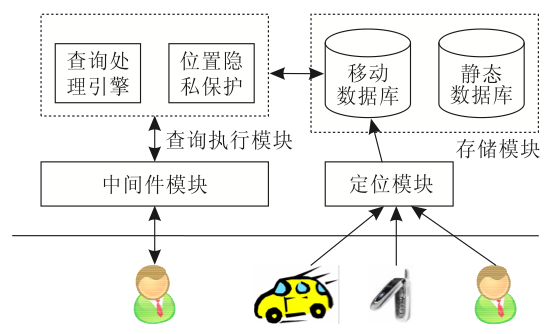
\includegraphics[bb=0 0 559 334, scale=0.45]{figure/fig_L10-2.png}
		\caption{LBS系统的架构}
		\label{fig:L10-2}
	\end{figure}

  通常,一个LBS服务提供商具备如下几方面特点\cite{L10}:高性能、可扩展性、高可靠性、实时性、移动性、开放性、安全性和互操作性。

	\subsubsection{基于空间信息网络的分布式思想的平台架构}
   刘丹、彭黎辉利用基于空间信息网络(spatial information grid, SIG)的分布式思想对空间位置服务平台的架构进行了模型设计和实现,完成了地图数据和定位查询的分布式存储和检索\cite{L08}。该平台服务满足开放位置服务(Open Location Service, 简称OpneLS)规范,利用XML进行信息编码,通过HTTP进行数据传输。同时,还针对定位信息的更新和传递提出了一种新的基于Push的主动通知机制,提供与各种定位接口的数据转换和消息处理能力,高效地实现了位置应用和服务平台之间地消息传递。

	\begin{figure}[htbp]
		\centering
		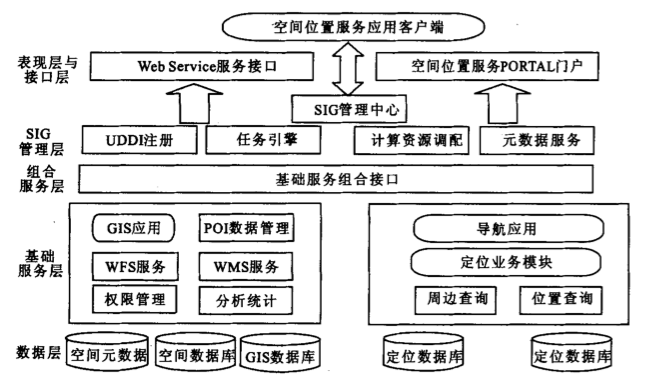
\includegraphics[bb=0 0 647 384, scale=0.45]{figure/fig_L08-4.png}
		\caption{SIG分布式架构}
		\label{fig:L08-4}
	\end{figure}

	LBS面向的空间数据量通常很大,涵盖的范围也不等,而SIG分布式架构网络化地设计和管理思想,可以有效地组织和管理这些数据,将各不同地域的数据托管在相应服务子站点服务器上,同时,这也很好的降低了用户集中访问同一台服务器造成的数据拥塞情况的发生。然而它也存在一定的缺点,分布式的平台架构在成本和管理力度上,则是一般中小企事业难以承受的。

	\subsubsection{基于J2EE的平台架构}
  蒋郁、刘伟平等人在LBS平台的设计过程中参考J2EE结构模型,并采用了组件式的设计方式,将整个平台划分成综合管理模块、GIS地理信息处理模块、接口层处理模块三大部分。此外,每个功能子模块独立封装,并对外提供统一规定的接口函数以供调用\cite{L06}。其中,综合处理模块作为整个平台的核心,负责将移动终端和业务服务联系起来,使移动用户获得所需的业务服务,其次还有用户认证、注册、计费等管理;GIS地理信息处理模块负责提供管理和处理大容量地图数据;LBS接口层处理模块负责和外部网络进行通信,使平台能在多种网络情况下运行,并且获得定位信息。基于J2EE开发模式的LBS平台系统工作流程如图\ref{fig:L06-2}所示:

	\begin{figure}[htbp]
		\centering
		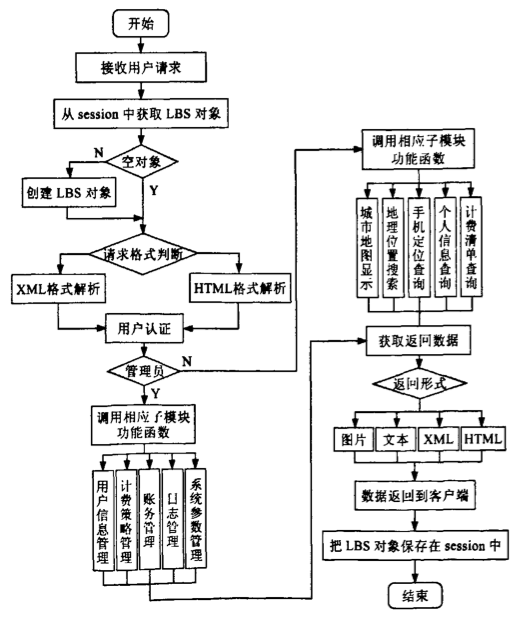
\includegraphics[bb=0 0 516 621, scale=0.45]{figure/fig_L06-2.png}
		\caption{基于J2EE开发模式的LBS平台系统工作的数据流程}
		\label{fig:L06-2}
	\end{figure}

  基于J2EE结构模型而设计实现的LBS系统平台,由于采用跨平台编程语言Java实现,所以具有良好的可移植性、可扩展性和平台无关性。另外,采用XML作为数据的统一格式,为不同平台的开发提供了方便。Jae-Chul Kim等人提出的平台架构也采用了XML作为数据的描述语言\cite{L13}。采用Web服务架构的平台,可以使得客户端的开发不受限于编程语言。

	\subsubsection{基于SOA的面向服务LBS}
  邹永贵、王剑提出了将SOA(Service-oriented Architecture,面向服务架构)架构运用于LBS,结合中间件技术,运用开放的Web服务技术,较好地解决了用户访问方式多样、异构兼容性不足和开发维护不易等问题\cite{L09}。

	\begin{figure}[htbp]
		\centering
		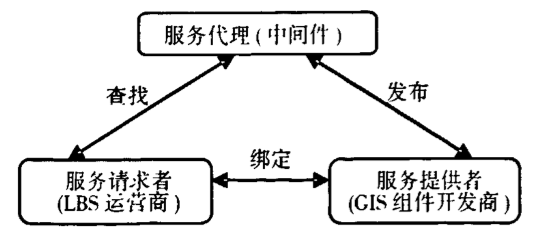
\includegraphics[bb=0 0 544 244, scale=0.45]{figure/fig_L09-2-1.png}
		\caption{面向服务的LBS定位服务平台构建模型}
		\label{fig:L09-2-1}
	\end{figure}

	\begin{figure}[htbp]
		\centering
		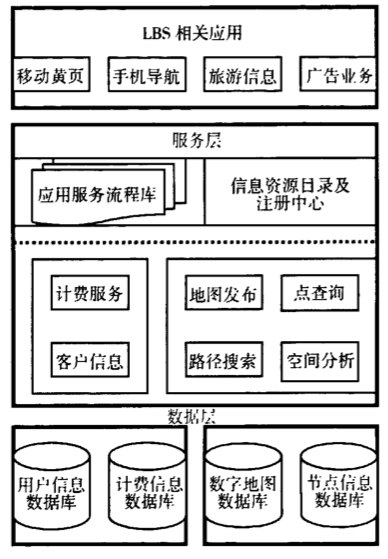
\includegraphics[bb=0 0 388 559, scale=0.45]{figure/fig_L09-2-2.png}
		\caption{面向服务的LBS定位服务平台架构}
		\label{fig:L09-2-2}
	\end{figure}

	从系统开发的角度来说,由于构建的LBS平台引入了中间件,所以只要求运营开发商具备一般的系统开发能力即可,开发的技术难度较小。GIS平台及相关硬件不需要运营商承担,因此开发成本也大为降低。同时,由于使用了基于XML的统一接口,所以开发灵活度也很高。

	而从系统应用角度来说,运营商只需要关注上层应用的日常运行和运营服务平台及流程服务器的更新,而底层包含核心应用模块的中间件则是由各GIS开发商负责的。这很大程度地降低了运营商对系统的运营成本和维护力度。

	\subsubsection{其它架构和方法}
  除了以上几种主流的架构方法外,还存在一些研究人员提出的其它架构方法,包括Aaron等人提出的一个开放式的基于SAGESS(Spatial Application Generic Environment System Standards,空间应用通用环境管理体系标准)的架构,以通过无线网络向用户提供富文本智能地图\cite{L05};W. Ait Cheik Bihi等人提出的TransportML\cite{L03};Rui Cheng等人提出的采用GIS、LBS、J2ME技术和地理数据结合而产生的平台:iZone,该平台可以为智能手机提供许多社交网络相关的服务\cite{L11};Paul J. Kuhn提出的LCBS\cite{L04}。

	\subsection{数据更新和获取}
  LBS的另一个重要服务便是信息服务,信息服务有源数据、信息有效期限、受众目标、位置依赖情况四个影响因素\cite{D06},改变其中任何一个都将影响到服务质量的好坏。用户在使用提供LBS技术的应用时,可能需要偶尔地,甚至随时随地地更新自己所在位置的相关信息,比如路径导航服务,就需要实时地对用户的当前位置进行更新,并同时获取道路交通情况信息。而如何处理数据的更新和获取,以及如何提升数据抓取的效率问题上,正是时下研究的热点之一。
   
  在数据更新方面,Suleiman Almasri等人提出的基于区域的更新机制\cite{L12},将一张大的地图划分成若干小的区域,用户只需下载自己所在位置的区域地图,所以,该更新机制可以大量减少信息传输量,很好的控制了网络带宽的使用,不仅提升了LBS性能,也最大限度地降低了用户设备的内存使用和功率消耗情况。

  在获取数据方面,各种数据挖掘技术已被广泛应用于从庞大且复杂的数据中获取到有价值的信息之中\cite{D09}。由于LBS系统的终端设备处理能力较低,显示屏幕较小,再加上无线数据网络带宽不足,因此无法浏览整个Web页面。采用信息抽取技术可以将用户感兴趣的信息提取出来,再发送给用户终端,有效地解决上述问题\cite{D11}。信息的过滤抽取可以减少冗余信息的传输,从而减少带宽的使用,提升数据的传输效率。随着移动技术地飞速发展,海量数据的传输也将变得容易,然而,对于用户来说,获取到真正有用的数据才是最重要的。通过信息抽取技术,所有发送到用户终端的数据都将根据用户所在位置和位置相关的信息进行过滤。用户还可以自定义信息的类别,以保证获取到自己更需要的信息,而不仅仅是位置相关的导航信息,而这也将为用户旅行在外提供更多方便和乐趣\cite{D10},此外,还可以为用户提供自动新闻概要服务\cite{D02}。

	\begin{figure}[htbp]
		\centering
		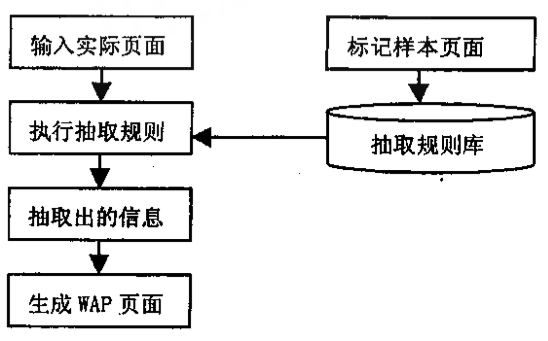
\includegraphics[bb=0 0 548 341, scale=0.45]{figure/fig_D11-2.png}
		\caption{基于LBS的信息抽取体系结构}
		\label{fig:D11-2-1}
	\end{figure}

  也因此,有人提出基于上下文和位置的服务(context and location bsed service)\cite{D05},为用户提供更个性化的自定义设置,从而提供更好的用户搜索查询体验(包括同一相关集群下的分组服务\cite{D05}、基于位置的抓取和推送服务\cite{D04})。

  Kahkashan Tabassum等人研究讨论了不同情形下,分布式处理位置相关的连续查询请求中遇到的各种挑战\cite{D08},并介绍了可以采用缓存和预加载技术,加大数据和查询结果的重用度,从而加快访问和响应的速度。另外,Shiow yang Wu等人提出的数据管理方法\cite{D06},也恰当地采用了缓存技术来提升LBS的效率。

  上述都是室外基于位置获取信息的一些技术方法,而现如今,室内的定位技术(如Kuofong Kao等人提出的通过将接入点作为信号强度数据采集器来实现室内的基于位置的服务\cite{D03})也在不断地被研究和实现,以适应今后不断增加的精度需求。

	\subsection{用户隐私}
  由于位置信息本身就易受伪造攻击(forging attacks),所以必须使用额外的机制以验证其完整性\cite{P04}。与此同时,保护用户的位置隐私也显得非常必要。位置隐私分为两类\cite{P02}:(1)敏感位置隐私,即用户对于所处位置比较敏感,希望自己的位置不被暴露;(2)位置-ID隐私,即攻击者能结合其它信息,根据用户的位置推断出用户的ID,导致用户的查询内容被暴露,此时用户对位置信息并不敏感,对查询内容是敏感的。

  隐私保护技术需要在保护隐私的同时,兼顾对应用的价值以及计算开销。通常可以从隐私保护度、数据缺损和算法性能三方面对隐私保护技术进行度量\cite{P01}。目前,一些实际可行的隐私保护方法已经得到研究并采用,比如基于二项式混合的位置匿名法\cite{P03}、基于点对点的隐蔽算法\cite{P05}、连续请求下的位置匿名方法\cite{P02}以及位置匿名化技术\cite{P01}等。各种隐私方法都有各自的不同特点,在不同需求下得到的效果也不尽相同。当针对特定数据实现隐私保护且对计算开销要求比较高时,基于数据失真的隐私保护技术更加适合;当更关注于对隐私的保护甚至要求实现完美保护时,则应该考虑基于数据加密的隐私保护技术,但代价是较高的计算开销(在分布式环境下,还会增加通讯开销)\cite{P01}。

	\subsection{本章小结}
  本章介绍了包括基于空间信息网络的分布式思想的平台架构、基于J2EE的平台架构、基于SOA的面向服务LBS等在内的LBS相关服务架构,并分析了数据更新和获取、用户隐私等关键技术。


	\section{客户端游戏设计与实现}
	\subsection{游戏设计概要}
  鉴于国内外LBS技术的研究和发展现状,在采用以LBS为核心技术的基础上,实现口袋妖怪类游戏的服务端和客户端的设计与实现。通过将现实世界中的地理位置与游戏虚拟世界相结合,开发基于位置服务的口袋妖怪类游戏。该游戏以经典口袋妖怪游戏为原型,运行于iOS平台上,并且结合了位置服务,口袋妖怪分布在真实的世界中。在不同的城市、国家,用户可以遇到不同的口袋妖怪。

	\subsection{开发环境}
  游戏客户端运行于iOS平台上,编程语言为Objective-C,采用Xcode v4.2进行项目管理和开发。
  服务端运行于Amazon EC2 Ubuntu 11.10系统实例上,编程语言为Python,采用Vim进行项目管理和开发。

	\subsection{客户端主要设计模式}
  游戏客户端采用Cocoa框架,结合MVC(Model-View-Controller,模型-视图-控制器)和单例(singleton)设计模式。

	\subsubsection{MVC}
  客户端开发采用MVC的设计模式,将展示层和逻辑层分离,以方便项目管理和后期的游戏逻辑修改。

  MVC是一种设计模式,它结合了策略(strategy)模式、合成(composite)模式、观察者(observer)模式等几种最基本的设计模式。MVC通过对自身基本部分分离的同时也赋予了各个基本部分应用的功能。

  MVC设计模式是软件工程中的一种软件架构模式,把软件系统分为三个基本部分:模型(Model)、视图(View)和控制器(Controller)。MVC模式的目的是实现一种动态的程式设计,使后续对程序的修改和扩展简化,并且使程序某一部分的重复利用成为可能。除此之外,此模式通过对复杂度的简化,使程序结构更加直观。软件系统通过对自身基本部份分离的同时也赋予了各个基本部分应有的功能。MVC设计模式各模块功能如下:

  \begin{enumerate}
    \item 视图(View):界面设计人员进行图形界面设计。
    \item 模型(Model):程序员编写程序应有的功能(实现算法等等)、数据库专家进行数据管理和数据库设计(可以实现具体的功能)。
    \item 控制器(Controller):负责转发请求,对请求进行处理。
  \end{enumerate}

  传统MVC设计模式下各模块交互图如下:

  \begin{figure}[htbp]
		\centering
		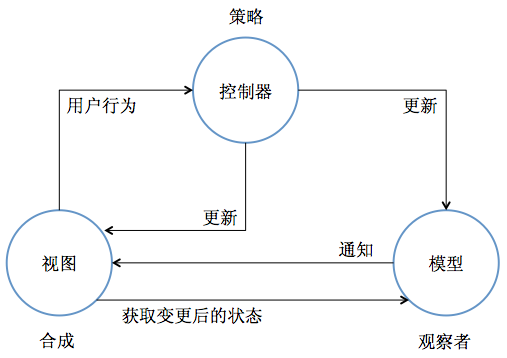
\includegraphics[bb=0 0 548 341, scale=0.45]{figure/fig_n01.png}
		\caption{传统MVC设计模式下各模块交互图}
		\label{fig:n01}
	\end{figure}

  而Cocoa框架提出尽量保持视图和模型的重用,避免视图和模型之间的交互,转而让控制器来完成,从而保持视图和模型之间的独立,也增强了可重用度。改进的MVC设计模式下各模块交互图如下:

  \begin{figure}[htbp]
		\centering
		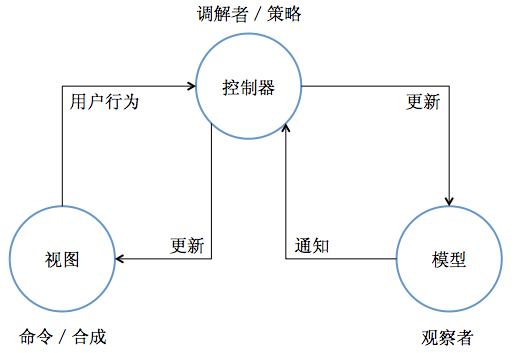
\includegraphics[bb=0 0 548 341, scale=0.45]{figure/fig_n02.png}
		\caption{Cocoa框架中的MVC设计摸下各模块交互图}
		\label{fig:n02}
	\end{figure}

  在该设计模式中,控制器将调解者(mediator)模式和策略模式进行了合并,从而调解视图和模型双向的数据流动。而通过视图对模型状态的变更,也就通过控制器来传达。另外,视图还通过实现Cocoa框架下的对象-行为(target-action)机制,结合了命令模式和合成模式。\cite{iOSLIB} 

	\subsubsection{单例设计模式}
  单例模式,也叫单子模式,是一种常用的软件设计模式。在应用这个模式时,单例对象的类必须保证只有一个实例存在。许多时候整个系统只需要拥有一个的全局对象,这样有利于我们协调系统整体的行为。比如在某个服务器程序中,该服务器的配置信息存放在一个文件中,这些配置数据由一个单例对象统一读取,然后服务进程中的其他对象再通过这个单例对象获取这些配置信息。这种方式简化了在复杂环境下的配置管理。

  实现单例模式的思路是:一个类能返回对象一个引用(永远是同一个)和一个获得该实例的方法(必须是静态方法,通常使用getInstance这个名称);当我们调用这个方法时,如果类持有的引用不为空就返回这个引用,如果类保持的引用为空就创建该类的实例并将实例的引用赋予该类保持的引用;同时我们还将该类的构造函数定义为私有方法,这样其他处的代码就无法通过调用该类的构造函数来实例化该类的对象,只有通过该类提供的静态方法来得到该类的唯一实例。\cite{WIKI}

	\subsection{总体设计与实现}
	\subsubsection{视图层次关系}
  如图所示为客户端视图整体层次关系(各视图均对应含有一个控制器,比如MainView对应的控制器为MainViewController):

  \begin{figure}[htbp]
		\centering
		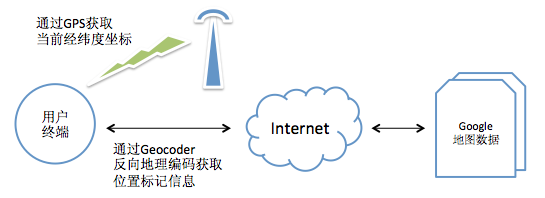
\includegraphics[bb=0 0 548 341, scale=0.45]{figure/fig_n03.png}
		\caption{视图整体层次关系}
		\label{fig:n03}
	\end{figure}

  MainView为主视图,它包括五个子视图:LoginTableView(登录视图)、HelpView(帮助视图)、MapView(地图)、GameMainView(游戏主视图)、CenterMenuUtilityView(主菜单视图)。其各功能如下:

  \begin{enumerate}
		\item LoginTableView:当用户session无效时显示给用户,提供第三方验证服务进行登;
		\item HelpView:用户帮助视图;
		\item MapView:地图,用户可查看自己所在位置,以及周边口袋妖怪情况等信息;
		\item GameMainView:游戏战斗主视图,当用户遇到野生口袋妖怪时,进入战斗场景;
		\item CenterMenuUtilityView:主菜单视图,包含六个子菜单:PokedexTableView(图鉴列表视图)、SixPokemonsTableView(用户所带口袋妖怪列表视图)、BagTableView(背包列表视图)、TrainerCardView(用户信息视图)、StoreTableView(商店视图)、SettingTableView(设置视图)。
  \end{enumerate}

  此外,GameMainView还包含一系列子视图,其层次关系如图所示:

  \begin{figure}[htbp]
		\centering
		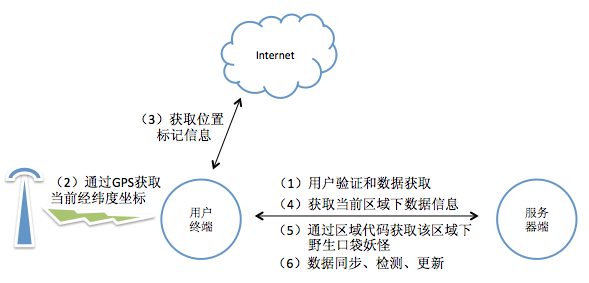
\includegraphics[bb=0 0 548 341, scale=0.45]{figure/fig_n04.png}
		\caption{GameMainView子视图层次关系}
		\label{fig:n04}
	\end{figure}

  所有视图对应的控制器调解视图的显示与更新、数据模型的获取与更新,以及视图与模型之间的通信。

	\subsubsection{数据模型}
  模型(在Cocoa中也称为entity,实体)主要有:Trainer(训练师,即用户)、TrainerTamedPokemon(训练师捕获的口袋妖怪)、WildPokemon(野生口袋妖怪)、Pokemon(口袋妖怪)、BagItem(背包物品)、Region(区域)、Move(口袋妖怪技能)、Ability(口袋妖怪特性)。

  Trainer、TrainerTamedPokemon、WildPokemon为动态模型,控制器可以检索当前相关数据,并对其进行更新后保存。而Pokemon、BagItem、Move、Ability为静态模型,控制器只检索相关数据,不对其进行更新。

  Trainer、TrainerTamedPokemon、WildPokemon模型相关类图如下:

  \begin{figure}[htbp]
		\centering
		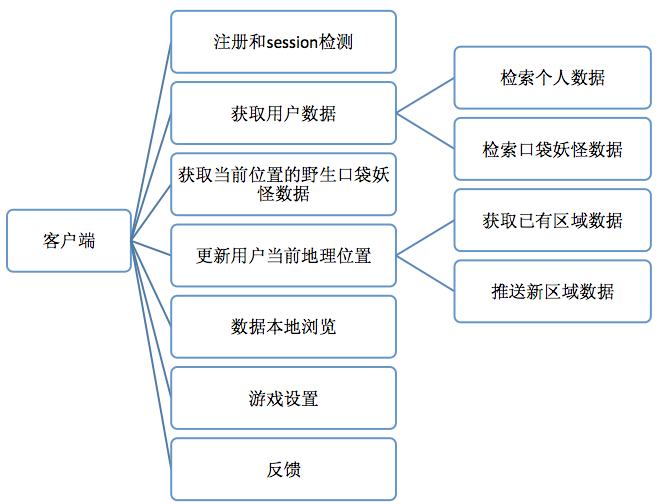
\includegraphics[bb=0 0 548 341, scale=0.45]{figure/fig_n05.png}
		\caption{Trainer模型相关类图}
		\label{fig:n05}
	\end{figure}

  \begin{figure}[htbp]
		\centering
		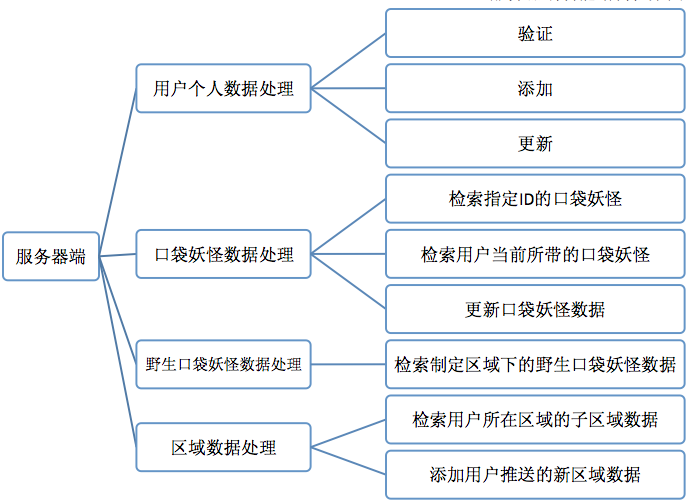
\includegraphics[bb=0 0 548 341, scale=0.45]{figure/fig_n06.png}
		\caption{TrainerTamedPokemon模型相关类图}
		\label{fig:n06}
	\end{figure}

  \begin{figure}[htbp]
		\centering
		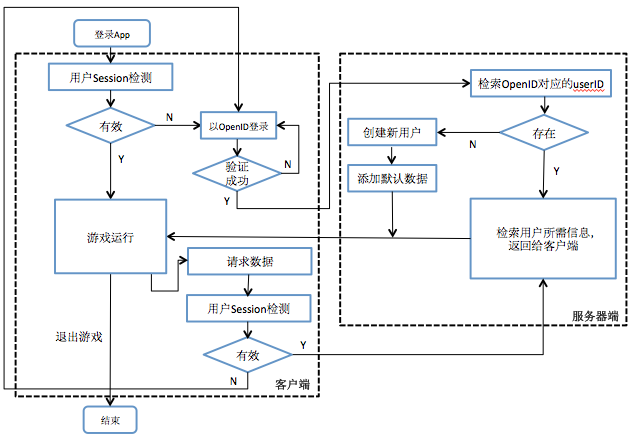
\includegraphics[bb=0 0 548 341, scale=0.45]{figure/fig_n07.png}
		\caption{WildPokemon模型相关类图}
		\label{fig:n07}
	\end{figure}

  类(category)为Objective-C中包含的特殊的类扩展方式,即该类在拥有相同的属性和方法的同时,可以添加更多方法(但不可添加属性),从而达到扩展类的作用,而类名不变。比如Trainer类,其扩展类为Trainer+DataController类(可被称为模型控制器),前者的方法只负责数据的增加、删除和更新,而后者在前者的基础上添加了数据检索相关方法,为其它控制器提供了方便的接口,也提升了重用度。在具体编程中,只需要加入Trainer+DataController.h文件,然后便可以对Trainer类使用扩展的方法了。类似的,TrainerTamedPokemon和WildPokemon也进行了相应的扩展。

  TrainerTamedPokemon和WildPokemon模型中属性pokemon为Pokemon类,关系为一对一。Pokemon模型为静态模型,只提供数据索引,其相关类图如下:

  \begin{figure}[htbp]
		\centering
		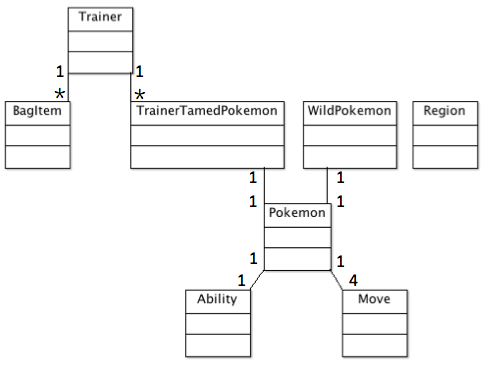
\includegraphics[bb=0 0 548 341, scale=0.45]{figure/fig_n08.png}
		\caption{Pokemon模型相关类图}
		\label{fig:n08}
	\end{figure}

  而对于BagItem、Move、Ability,可分别通过SID号索引静态数据。

  Region为游戏提供基于位置的相关数据,具体数据处理机制将在“基于位置服务的口袋妖怪分布机制”一章中进行详细的介绍。其模型相关类图如下:

  \begin{figure}[htbp]
		\centering
		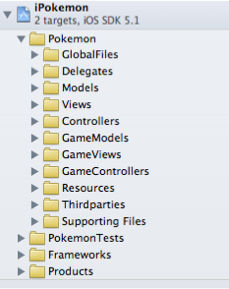
\includegraphics[bb=0 0 548 341, scale=0.45]{figure/fig_n09.png}
		\caption{Region模型相关类图}
		\label{fig:n09}
	\end{figure}

  Region+DataController类同样为Region进行了扩展,为检索和同步数据提供了简单的接口。

	\subsubsection{单例}

  在客户端中,为方便游戏的全局控制,设计了一系列单例:PMAudioPlayer、LoadingManager、ServerAPIClient、OAuthManager、PMLocationManager、TrainerController、WildPokemonController,以及GameStatusMachine、GameSystemProcess、GamePlayerProcess、GameEnemyProcess。

  PMAudioPlayer、LoadingManager、ServerAPIClient、OAuthManager、PMLocationManager各功能如下:

  \begin{enumerate}
		\item PMAudioPlayer:对背景音乐、音效进行全局控制;
		\item LoadingManager:控制同步、异步加载;
		\item ServerAPIClient:提供与服务端交互的接口,包括获取和更新用户ID、数据,区域信息等;
		\item OAuthManager:提供用户验证、session检测、注销等接口;
		\item PMLocationManager:监听用户在地理位置上的移动,适时地更新地理位置标记信息。
  \end{enumerate}

  TrainerController提供当前用户所有包括个人信息、背包数据、捕获的口袋妖怪相关数据等在内的数据处理接口,此外还包括用户的验证、与服务端数据的同步等接口。其相关类图如下:

  \begin{figure}[htbp]
		\centering
		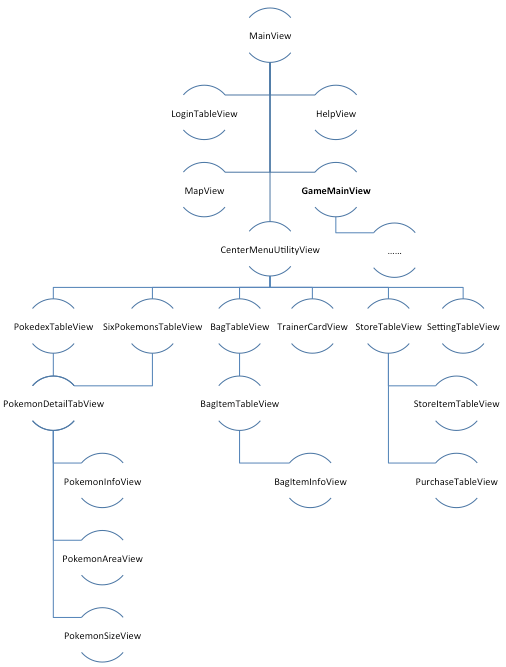
\includegraphics[bb=0 0 548 341, scale=0.45]{figure/fig_n10.png}
		\caption{TrainerController单例相关类图}
		\label{fig:n10}
	\end{figure}

  WildPokemonController根据PMLocationManager获取的用户当前地理位置数据,生成相应的野生口袋妖怪。同时,它包含与服务端数据交互的私有接口。其相关类图如下:

  \begin{figure}[htbp]
		\centering
		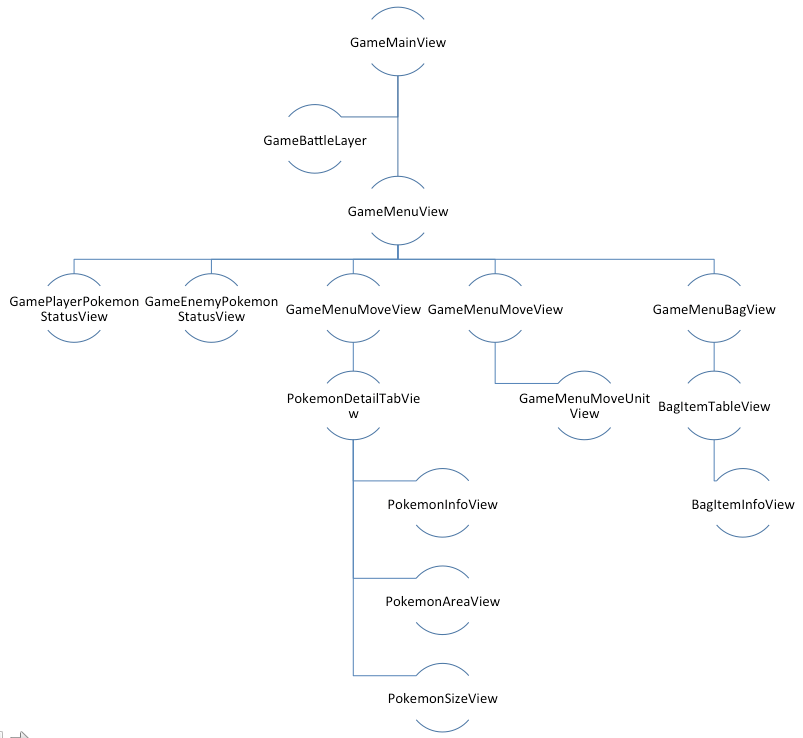
\includegraphics[bb=0 0 548 341, scale=0.45]{figure/fig_n11.png}
		\caption{WildPokemonController单例相关类图}
		\label{fig:n11}
	\end{figure}

  GameStatusMachine为在战斗模式下的状态机,对游戏战斗的回合进行控制。而GameSystemProcess、GamePlayerProcess、GameEnemyProcess均为CCNode子类,包含update:方法来更新游戏,三者分别为系统处理器、用户(玩家)处理器、敌人(野生口袋妖怪)处理器,在游戏回合中各自监听和处理自己的事件。

	\subsection{游戏开发成果}
  游戏客户端有简体中文和英文两个版本。

	\subsubsection{基本功能}

  \begin{enumerate}
    \item 可以根据你所在的位置出现不同的口袋妖怪
    \item 如果拥有精灵球,就可以捕获口袋妖怪
    \item 应用可以在后台运行,当出现野生口袋妖怪时,会收到应用的推送信息
    \item 可以使用回复类治疗口袋妖怪
    \item 内置商店,可购买物品
    \item 以及更多原口袋妖怪游戏中存在的一些功能
  \end{enumerate}

	\subsubsection{界面设计}
  游戏客户端界面主要采用Cocoa框架下的UIKit库进行编写。主要视图示例如下:

  \begin{figure}[htbp]
		\centering
		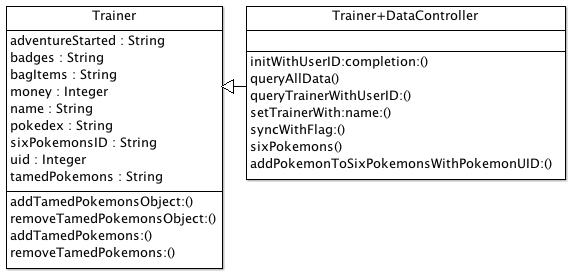
\includegraphics[bb=0 0 548 341, scale=0.45]{figure/fig_n12.png}
		\caption{主视图和主菜单视图}
		\label{fig:n12}
	\end{figure}

  \begin{figure}[htbp]
		\centering
		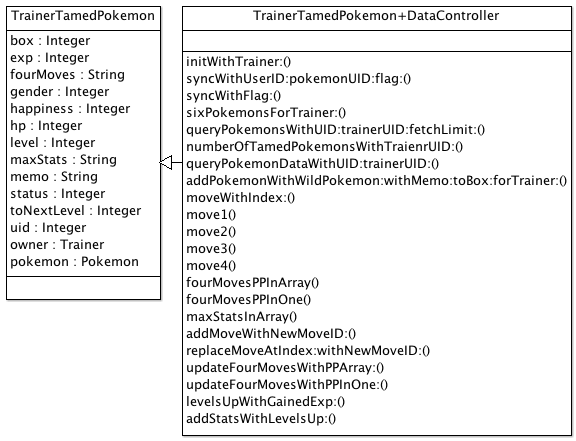
\includegraphics[bb=0 0 548 341, scale=0.45]{figure/fig_n13.png}
		\caption{TrainerController单例相关类图}
		\label{fig:n13}
	\end{figure}

  \begin{figure}[htbp]
		\centering
		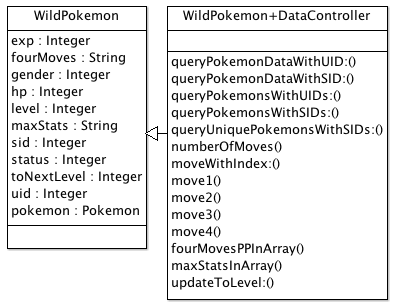
\includegraphics[bb=0 0 548 341, scale=0.45]{figure/fig_n14.png}
		\caption{口袋妖怪图鉴视图和信息视图}
		\label{fig:n14}
	\end{figure}

  \begin{figure}[htbp]
		\centering
		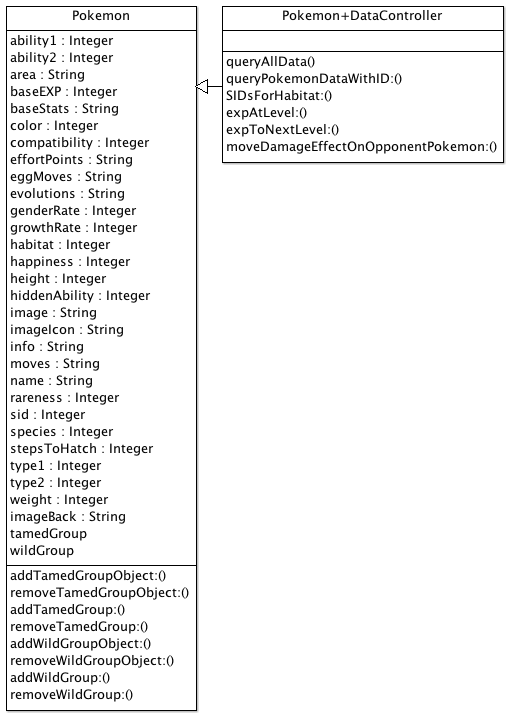
\includegraphics[bb=0 0 548 341, scale=0.45]{figure/fig_n15.png}
		\caption{背包视图和背包项视图}
		\label{fig:n15}
	\end{figure}

  \begin{figure}[htbp]
		\centering
		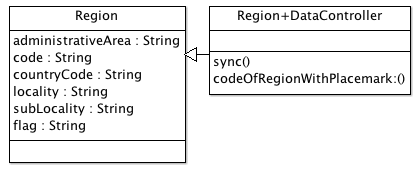
\includegraphics[bb=0 0 548 341, scale=0.45]{figure/fig_n16.png}
		\caption{商店视图和设置页视图}
		\label{fig:n16}
	\end{figure}

  \begin{figure}[htbp]
		\centering
		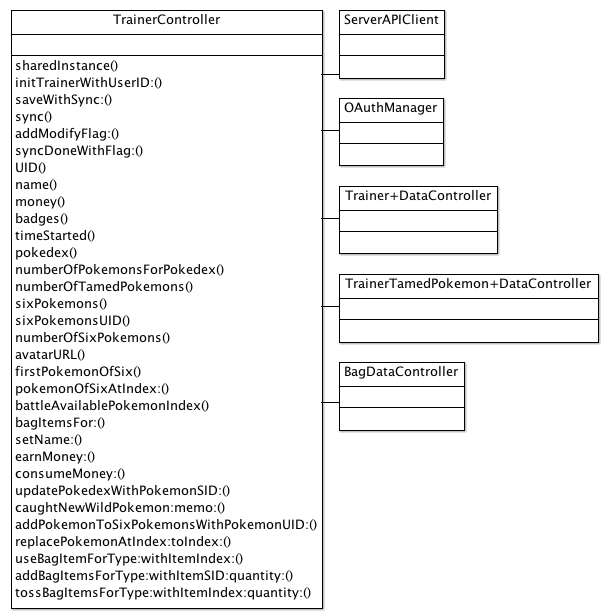
\includegraphics[bb=0 0 548 341, scale=0.45]{figure/fig_n17.png}
		\caption{战斗场景视图和口袋妖怪替换视图}
		\label{fig:n17}
	\end{figure}

	\subsubsection{操作说明} 
  游戏主视图中间的按钮是游戏的主按钮,用户可以通过它打开主菜单。而在它之上的按钮是地图按钮,默认为红色,也就是说位置服务被禁用,用户可以通过按住该按钮保持3秒来开启位置服务,然后按钮会变为白色。

  开启位置服务后,用户可以根据自己当前位置的不同遇到不同的野生口袋妖怪。当有野生口袋妖怪出现时,主按钮会改变状态以示提醒用户。通过按下提醒状态下的主按钮,游戏便加载战斗场景。

  在战斗场景中,用户可以做如下手势操作:

  \begin{enumerate}
    \item 向右滑动手指:展开技能窗口
    \item 向坐滑动手指:展开背包窗口
    \item 向上滑动手指:展开你的口袋妖怪的状态栏
    \item 向下滑动手指:展开野生口袋妖怪的状态栏
    \item 轻按底部按钮:展开口袋妖怪选择窗口,用于替换口袋妖怪
    \item 双指连续轻敲两下:尝试逃离战斗
  \end{enumerate}

	\subsection{本章小结}
  本章介绍了游戏客户端设计与实现的方法,将客户端开发过程中遇到的问题和解决方案,以及最后开发成果进行一个详细的介绍。
  

	\section{Web服务和LDAP(Lightweight Directory Access Protocol)服务}
	\subsection{弹性云存储服务:EC2}
  本项目Web服务采用Amazon提供的弹性云计算服务(Elastic Compute Cloud,简称EC2)。Amazon EC2是一个提供可调整云计算能力的Web服务。它的简单Web服务接口允许用户轻松获取和配置云计算性能,在提供高效稳定的服务环境的同时,还向用户提供了计算资源的完全控制权限。Amazon EC2可减少用户获取和启动新的服务器实例所需的时间,从而可以快速地改变(不管是增加还是减少)计算性能需求的变化。\cite{AWS}

	\subsection{键值存储服务:Redis}
  Redis是一个键值(key-value)存储服务系统,全称REmote DIctionary Service。同Memcached类似,它支持存储包括string(字符串)、list(链表)、set(集合)、zset(有序集合)和hash(哈希)在内的值类型。这些数据类型都支持push/pop、add/remove及交并集和差集的操作,而且这些操作都是原子性的。在此基础上,redis还支持各种不同方式的排序。为了保证数据读取效率,redis将数据都缓存于内存中,然后周期性的把更新的数据写入到磁盘(或者可以选择将修改操作追加到日志文件),并且还可在此基础上实现主从(master-slave)同步,从而有效降低灾难性的数据损坏或丢失情况所带来的损失。

  虽然键值数据库还没有完全成熟,但它的确为开发分布式和弹性Web应用提供了很好的选择\cite{REDIS}Persisting Objects in Redis Key-Value Database。Redis主体结构就是实现一个hash table,它定位于一个内存数据库,正是由于内存的快速访问特性,才使得Redis能够有如此高的性能,能够轻松处理大量复杂的数据结构。

  而对于持久化存储问题,redis提供了RDB(Redis DB)快照和AOF(Append Only File)日志两种策略。

  \begin{enumerate}
		\item RDB快照:Redis支持将当前数据的快照存成一个数据文件的持久化机制。而一个持续写入的数据库如何生成快照呢。Redis借助了fork命令的copy on write机制。在生成快照时,将当前进程fork出一个子进程,然后在子进程中循环所有的数据,将数据写成为RDB文件。
      Redis的RDB文件不会坏掉,因为其写操作是在一个新进程中进行的,当生成一个新的RDB文件时,Redis生成的子进程会先将数据写到一个临时文件中,然后通过原子性rename系统调用将临时文件重命名为RDB文件,这样在任何时候出现故障,Redis的RDB文件都总是可用的。
      同时,Redis的RDB文件也是Redis主从同步内部实现中的一环。
		\item AOF日志:它是一个追加写入的日志文件。与一般数据库日志不同的是,AOF文件是可识别的纯文本,它的内容就是一个个的Redis标准命令。
      然而,如果每一条写命令都生成一条日志,那么AOF文件将会变得非常大。所以,Redis又提供了一个AOF Rewrite的功能,它将重新生成一份AOF文件,新的AOF文件中一条记录的操作只会有一次,而不像一份老文件那样,可能记录了对同一个值的多次操作。其生成过程和RDB类似,也是fork一个进程,直接遍历数据,写入新的AOF临时文件。在写入新文件的过程中,所有的写操作日志还是会写到原来老的AOF文件中,同时还会记录在内存缓冲区中。当重完操作完成后,会将所有缓冲区中的日志一次性写入到临时文件中。然后调用原子性的rename命令用新的AOF文件取代老的AOF文件。
  \end{enumerate}

  RDB和AOF操作都是顺序IO操作,性能都很高。而同时在通过RDB文件或者AOF日志进行数据库恢复的时候,也是顺序的读取数据加载到内存中,所以也不会造成磁盘的随机读。

  此外,redis还支持pipeline模式,其具体过程是客户端一次性发送N个命令,然后等待这N个命令的返回结果被一起返回,从而减少网络I/O次数。该模式下,服务端将命令结果放进queue,再返回给客户端。

  \subsection{服务端接口设计与实现}
  服务端以Python语言进行编写,采用轻量级Web服务框架Bottle构建Web服务,提供RESTful API。服务器托管于美国西部的加利福尼亚洲,Amazon EC2上运行64位Ubuntu 11.10系统实例,开放22端口(用于管理员通过SSH进行连接管理服务器)和8080端口(用于客户端访问API)。考虑到费用和服务需求之间的关系,选择采用最低性能的实例(Micro Instance),提供613MB内存。

  用户数据使用Redis v2.4进行存储,采用Redis Python Client(提供Python访问Redis数据的接口)进行数据交互操作。

  主要API设计如下:

  \begin{enumerate}
		\item /id:ID,获取已验证用户的ID
		\item /u:user,获取用户数据
		\item /uu:update user,更新用户数据
		\item /6pm:six PokeMons,获取用户所带口袋妖怪数据
		\item /pd:PokeDex,获取用户口袋妖怪图鉴数据
		\item /upm:Update PokeMon,更新口袋妖怪数据
		\item /wpm:Wild PokeMon,获取用户当前区域下可能出现的野生口袋妖怪
		\item /r/<code>:Region,获取指定区域code的区域数据(code示例:CN:ZJ:HZ:XX:XX,下一章将详细说明)
  \end{enumerate}

  用户通过OpenID登陆Google Account,成功授权后,客户端发送请求到服务端,如果识别到为新用户,则通过redis的INCR操作,生成用户ID作为key,用户身份信息作为value,通过redis的SADD操作,将用户信息加入到用户集合中,同时为用户生成默认数据。之后用户可以直接通过识别信息(identity)来获取服务端用户数据、基于地理位置的口袋妖怪数据等。游戏运行的简单流程图如图所示:

  \begin{figure}[htbp]
		\centering
		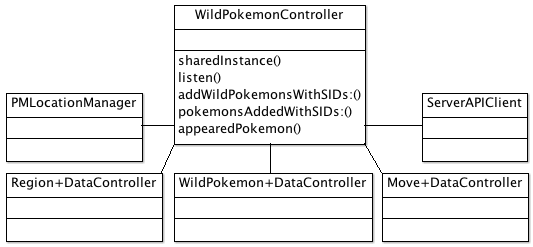
\includegraphics[bb=0 0 548 341, scale=0.45]{figure/fig_n18.png}
		\caption{游戏运行流程图}
		\label{fig:n18}
	\end{figure}

	\subsection{本章小结}
  本章介绍了服务端用到的主要服务:Amazon EC2和键值数据服务Redis,并对服务端接口的设计以及客户端和服务端的交互做了简单的介绍。


	\section{基于位置服务的口袋妖怪分布机制}
  游戏中,口袋妖怪在现实世界中的分布并不是一成不变的,它通过服务器采用算法每隔一定时间自动生成口袋妖怪分布图,映射到现实中。客户端(用户移动设备)通过一定时间间隔发送消息到服务端,询问是否有口袋妖怪。
  
  根据经纬度,可获得用户当前所在位置可能出现的野生口袋妖怪,另外也尽量考虑地形的影响,比如沿海城市出现水系口袋妖怪,沙漠地带出现岩石类口袋妖怪,等等。

	\subsection{反向地理编码}
  基于位置服务的数据往往是对应于用户当前位置在地球上的经纬度值,这些经纬度坐标值虽然可以很精确方便地应用与代码中,但是对于用户来说显得并不那么直观。相比坐标值,用户更容易了解与该地理位置相关的特殊信息,比如街道、城市、洲或者国家。\cite{iOSLIB}

  Cocoa框架下的Core Location库中包含Geocoder对象,该对象使用网络服务对经纬度和位置标记(placemark)进行相应的转换。而方向地理编码(reverse geocoding)就是将经纬度坐标转换成位置标记的过程。如图所示为反向地理编码流程示意图:

  \begin{figure}[htbp]
		\centering
		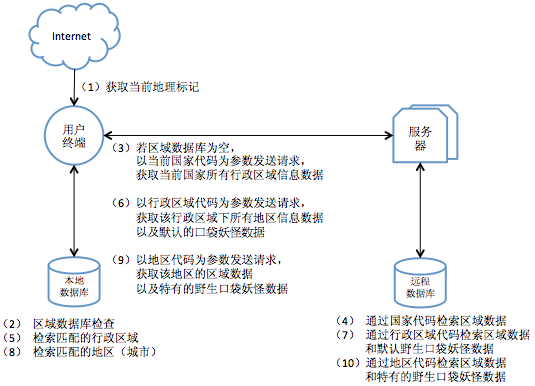
\includegraphics[bb=0 0 548 341, scale=0.45]{figure/fig_n19.png}
		\caption{反向地理编码流程图}
		\label{fig:n19}
	\end{figure}

	\subsection{数据信息搜集、匹配、处理和交互机制}
  通过反向地理编码获得的地理标记包含国家代码(ISOcountryCoude)、国家名(country)、邮政编码(postalCode)、行政区域名(administrativeArea)、地区名(locality)、次级地区名(subLocality)、是否为内陆水域(inlandWater)、是否为海洋(ocean)等信息。

  \begin{enumerate}
		\item 属性名 | 说明
		\item addressDictionary | 一个可读的连续地址字典
		\item administrativeArea | 行政区域名
		\item areasOfInterest | 与当前区域相关的有趣的地方
		\item country | 国家名称
		\item inlandWater | 内陆湖泊名称
		\item ISOcountryCode | 国家缩写代码
		\item locality | 地区(城市)名称
		\item location | 一个包含经纬度坐标的CLLocation对象
		\item name | 地理标记名
		\item ocean | 海洋名称(如果所在处为海洋的话)
		\item postalCode | 邮政编码
		\item region | 地理区域范围
		\item subAdministrativeArea | 附加的行政区域信息(可无)
		\item subLocality | 次级地区名(可无)
		\item subThoroughfare | 附加街道信息
		\item thoroughfare | 街道名称
  \end{enumerate}
  地理标记(placemark)各属性和说明
  
  然而,这些信息也仅仅为显示给用户而设计,也就说,当用户发送请求后,获得的是自己所在位置对应经纬度坐标下的地理信息,然后显示在屏幕上。而如何确定用户所在处,这就需要对获得的信息进行相应的匹配来确定,但Apple并没有给出所有地理信息名称,所以需要通过用户来搜集地理信息名称,然后将更新好的地理信息存储到服务器,下次其它用户就可以获取该地理信息了。具体设计如下:

  客户端和服务端各包含一个区域数据库。客户端数据库(本地数据库)存储用户在当前省份下的区域信息,服务端数据库(远程数据库)存储全球区域信息。当用户登录客户端后,进行区域信息数据初始化工作:根据用户当前经纬度坐标,反向地理编码后获得区域信息,若本地数据库为空,则以国家代码(如中国的国家代码为CN)作为参数向服务端发送请求,获取该国家下所有行政区域(或省)信息数据。通过检索匹配的行政区域名获得的行政区域代码(如中国浙江省为CN:ZJ,不存在则以CN:XX代替),向服务器发送请求获得该行政区域下所有地区信息数据,同时获取分布于该行政区域下的默认口袋妖怪数据。再从本地数据库中检索匹配的地区名,若存在,则以国家和该行政区域代码(如中国浙江省对应的代码为CN:ZJ)作为参数向服务端发送请求,获取该区域对应的特殊口袋妖怪数据;若不存在,则统一采用默认代码(CN:XX:XX)作为索引的地区代码,向服务器获取分布于该国的默认口袋妖怪数据。

   \begin{figure}[htbp]
		\centering
		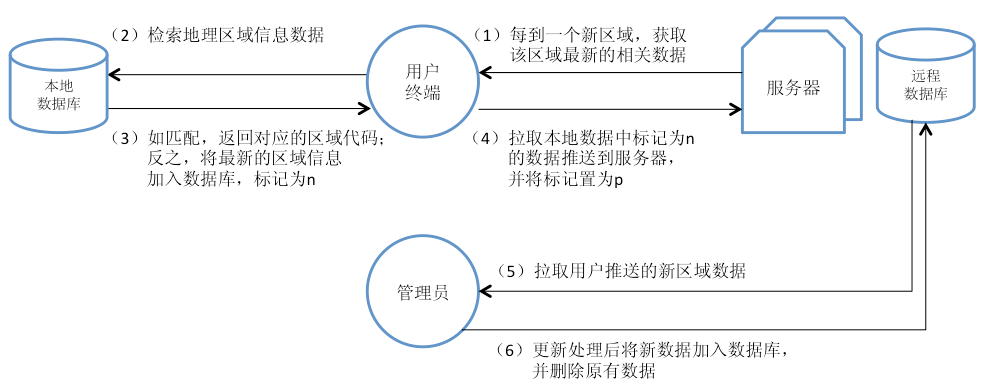
\includegraphics[bb=0 0 548 341, scale=0.45]{figure/fig_n20.png}
		\caption{客户端和服务端交互详细示意图}
		\label{fig:n20}
	\end{figure}

  之后,用户每到一个地方,向数据库索引匹配的数据,若存在,返回该地理位置对应的区域代码(如对应中国浙江杭州市余姚区CN:ZJ:HZ:YY),然后向服务器发送请求,获取该区域下特有的口袋妖怪数据;若不存在,则将该地理位置存入本地数据库,将flag参数设置为n(即新区域信息数据),然后在下次向服务器抓取数据的同时,将所有标记为n的区域信息数据发送给服务器,然后将标记重置为p(即区域信息数据以发送给服务器,下次不必再进行存储和发送工作)。

  远程数据库中,对未知行政区域信息,统一存储在国家代码下,比如,中国,获得未知的行政区域名:Heilongjiang(黑龙江),那么,对应在redis中的键值也就是:nre:CN => 'Heilongjiang Province',其中,nre代表新区域(New REgion)作为键前缀,nre:CN对应的值为一个集合。而对未知地区信息,则统一存储在行政区域对应代码下,比如,中国浙江,获得未知的地区名:Shaoxing(绍兴),那么,对应在redis中的键值也就是:nre:CN:ZJ => 'Shaoxing City'(同样,nre:CN:ZJ对应的值为一个集合)。

  管理员每隔一段时间对地理信息数据进行维护,抓取所有前缀为nre的键对应的集合,对每条数据进行更新,比如数据:nre:CN:ZJ => Shaoxing,更新后,记代码为CN:ZJ:SX。最后,将所有更新了的数据以re:CN:ZJ:SX => 'CN:ZJ:SX,Zhejiang Province,Shaoxing City'形式存储到数据库中,同时备份删除原先前缀为nre的键对应的数据。

  最后,对区域代码和对应的野生口袋妖怪ID进行键值匹配,设定对应区域下特殊的口袋妖怪。比如中国浙江省杭州市余杭区特有的野生口袋妖怪ID有1,2,3,则对应数据为wpm:CN:ZJ:HZ:YY => '1,2,3',其中,wpm代表野生口袋妖怪(Wild PokeMon)作为键前缀。

  \begin{figure}[htbp]
		\centering
		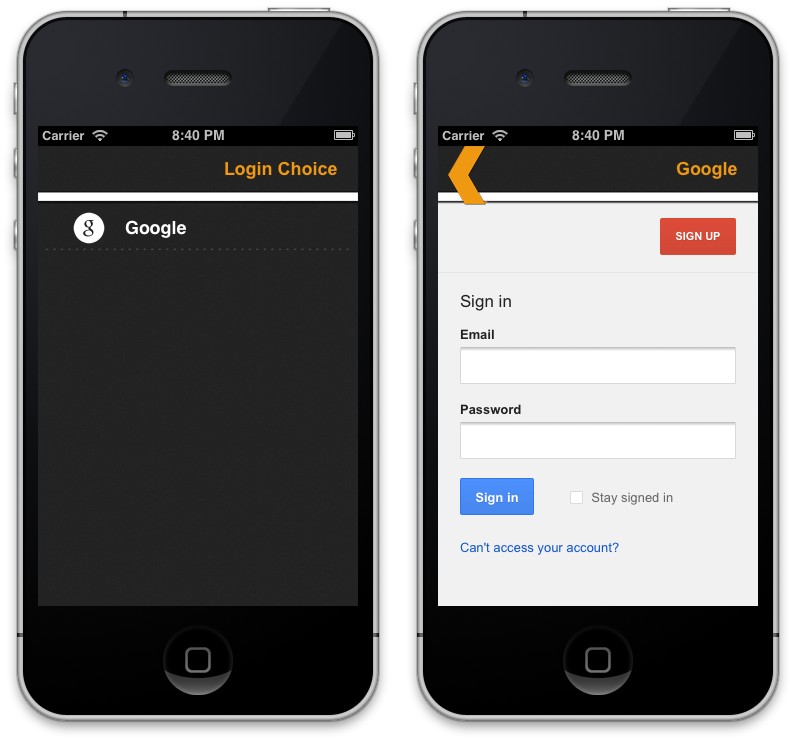
\includegraphics[bb=0 0 548 341, scale=0.45]{figure/fig_n21.png}
		\caption{地理信息数据更新示意图}
		\label{fig:n21}
	\end{figure}

  之后,其它用户在获取区域信息和对应的野生口袋妖怪时,便可以获取到最新的数据信息。

	\subsection{本章小结}
  本章主要介绍了反向地理编码技术在LBS中的运用,同时详细地描述了地理位置和野生口袋妖怪相关信息的搜索、匹配、处理和交互机制的设计与实现。


	\section{总结与展望}
	\subsection{总结}
  论文论述了LBS相关架构和基于位置服务的口袋妖怪类游戏客户端和服务端的设计与实现。客户端采用Cocoa框架,以Objective-C语言编写iPhone客户端游戏程序,通过将现有LBS技术应用于游戏中,将真实世界映射到游戏中,形成一个真实的口袋妖怪世界。采用CoreData作为客户端数据服务,Sqlite3作为数据库保存用户本地数据。服务端托管于Amazon EC2上,采用Python语言编写服务端程序,向客户端提供RESTful API,实现了用户验证、获取用户ID和数据、获取用户当前位置下特殊的野生口袋妖怪数据、更新区域位置数据等主要功能。采用键值数据服务Redis作为服务端数据库,鉴于其运行于内存上,所以拥有很高的性能,能够快速响应用户请求。在Redis的配置上,选择每隔一段时间将内存中的数据写入到磁盘,作为数据永久化保存策略。此外,所有客户端和服务端之间的通信,都采用异步编程,数据的传输对用户来说都是透明的。最后,实现了针对iOS平台的基于位置服务的口袋妖怪类游戏。

	\subsection{展望}
  口袋妖怪这款经典游戏深受游戏玩家喜爱,然而由于版权属于任天堂,所以后续开发需要加入自己设计的一套类口袋妖怪的角色和相应的数据,以此避免版权纠纷。Solomo(social-local-mobile,即社交、位置、移动)的应用模式正逐渐被人们肯定。毫无疑问,在位置服务和移动游戏的基础上加入社交元素,将吸引更多的玩家,而社交元素也正是后续考虑加入的。另外,也将加入多人对战、交易等模式,令游戏更具可玩性。相信这款基于位置服务的口袋妖怪类游戏也将深受玩家喜爱。


	\section{致谢}
  在论文完成之际,我要感谢在论文写作和研究期间给予我帮助的老师、同学和朋友们。
  首先要感谢我的指导教师王万良教授和徐新梨副教授。感谢两位在毕业设计期间给予我的悉心指导,为我提供了一个良好的工作和学习环境。他们一丝不苟的工作作风、严谨的治学态度和对工作无私的奉献精神,深深地影响了我,使我受益匪浅。
  再次感谢徐新黎副教授耐心地对我的论文提出修改意见。
  还要感谢我身边和异地的同学、朋友们对我的关心和帮助。
  最后感谢我的父母。感谢他们生活上对我无微不至的照顾与关怀,学业和事业上一如既往的支持与鼓励。
  

	% Import references datas
  \bibliography{references.bib}

	\end{CJK}
\end{document}
